\documentclass[10pt,a4paper]{article}
\usepackage[utf8]{inputenc}
\usepackage[italian]{babel}
\usepackage{amsmath}
\usepackage{amsfonts}
\usepackage{float}
\usepackage{amssymb}
\usepackage{xcolor}
\usepackage{graphicx}

% Per l'inserimento di codice OpenModelica
\usepackage{listings}
%% listings-modelica.cfg
%% Copyright 2014 Martin Sjoelund, Dietmar Winkler
%
% This work may be distributed and/or modified under the
% conditions of the LaTeX Project Public License, either version 1.3
% of this license or (at your option) any later version.
% The latest version of this license is in
%   http://www.latex-project.org/lppl.txt
% and version 1.3 or later is part of all distributions of LaTeX
% version 2005/12/01 or later.
%
% This work has the LPPL maintenance status `maintained'.
%
% The Current Maintainer of this work is Dietmar Winkler
%
% Code repository https://github.com/modelica-tools/listings-modelica
%
% This work consists of the file listings-modelica.cfg

\lstdefinelanguage{modelica}
{
  morekeywords=[1]{
    algorithm,and,annotation,as,assert,block,break,case,class,connect,connector,
    constant,constrainedby,der,discrete,each,else,elseif,elsewhen,encapsulated,
    end,enumeration,equality,equation,expandable,extends,external,failure,final,
    flow,for,function,guard,if,import,in,initial,inner,input,List,local,loop,
    match,matchcontinue,model,not,operator,Option,or,outer,output,package,parameter,
    partial,protected,public,record,Real,redeclare,replaceable,return,stream,
    subtypeof,then,Tuple,type,uniontype,when,while},
  morekeywords=[2]{true, false},
  % Do not make true,false keywords because fn(true,x, false ) shows up as fn(true,x, *false*)
  morekeywords=[3]{optimization,constraint}, % Optimica keywords
  morekeywords=[4]{objective,startTime,finalTime,initialGuess},
  sensitive=true,
  comment=[l]//,
  morecomment=[s]{/*}{*/},
  alsodigit={.,-},
  morestring=[b]',
  morestring=[b]",
}[keywords,comments,strings]

\definecolor{keywordcolor1}{rgb}{0,0,.4}
\definecolor{keywordcolor2}{rgb}{.90,0,0}
\definecolor{keywordcolor3}{rgb}{.4,0,.8}
\definecolor{keywordcolor4}{rgb}{0.5,0,0.5}
\definecolor{stringcolor}{rgb}{0.133,0.545,0.133}
% \definecolor{listingbgcolor}{rgb}{0.95,0.95,0.95}

\lstset{
  breaklines=true,
  language=modelica,
  basicstyle=\ttfamily,
  keywordstyle=[1]\color{keywordcolor1}\bfseries,
  keywordstyle=[2]\color{keywordcolor2},
  keywordstyle=[3]\color{keywordcolor3}\bfseries,
  keywordstyle=[4]\color{keywordcolor4},
  stringstyle=\color{stringcolor},
%  backgroundcolor=\color{listingbgcolor},
  framexleftmargin=5pt,
  xleftmargin=5pt,
  xrightmargin=5pt,
  showstringspaces=false
}

\newcommand{\code}[1]{\lstinline|#1|}
\newcommand{\modelica}[1]{\lstinline[language=modelica]|#1|}


\graphicspath{ {./images/} }
\author{Gianluca Mondini}
\title{Tesi (titolo da definire)}

\begin{document}

\begin{center}
\textbf{Attenzione: il seguente documento è ancora in fase di stesura, pertanto presenta sezioni abbozzate, incorrette ed incomplete.}
\end{center}

\maketitle

%\pagebreak

%\tableofcontents

%\pagebreak

\section{Obiettivo}

Implementazione dell'algoritmo di Lloyd per l'equidistribuzione di uno sciame di droni su un'area specifica.

È prevista la realizzazione di un modulo nell'ambiente \textit{OpenModelica} che permetta di simulare il suddetto algoritmo; più avanti verranno illustrate parti di codice e verranno fornite informazioni relative alla sua implementazione.

\section{Parole chiave}

Prima di procedere con la trattazione, è necessario indicare alcune parole chiave presenti in questo documento e nel codice dell'implementazione

\begin{description}
	\item[Drone] Velivolo che, nel nostro caso di interesse, è rappresentato come un punto bidimensionale
	\item[Area] Poligono convesso che delimita l'algoritmo;
	\item[Cella] Porzione di spazio alla quale appartiene un drone; la cella relativa ad un drone è l'insieme di punti dell'area per i quali, tra tutti i vari droni, quello appartenente alla cella è il più vicino
\end{description}

\section{Il drone e sue componenti}

Possiamo schematizzare, ai fini di questa trattazione, un \textit{drone} mediante 3 componenti: il \textit{centro fisico}, il \textit{controllo di volo} e il \textit{controllo della traiettoria}\footnote{da rivedere i nomi dei 3 componenti}

\begin{center}
\textbf{Inserire qui uno schemino che illustri i tre componenti del drone}
\end{center}

\subsection{Centro fisico}

Il centro fisico è un astrazione che rappresenta il rapporto del drone con il mondo esterno. Vengono quindi qui considerati parametri la massa, la velocità, l'accelerazione, la posizione, la rotazione, la velocità di rotazione dei motori e la potenza che viene fornita a questi.

\section{Algoritmo di Lloyd}

\subsection{Introduzione}

L'algoritmo di Lloyd, conosciuto anche con il nome di \textit{iterazione di Voronoi}, è un algoritmo che permette di suddividere un'area in celle convesse uniformemente dimensionate.

L'algoritmo di Lloyd è implementato mediante iterazioni continue dell'algoritmo di Voronoi.

\subsection{Descrizione}

L'algoritmo esegue ripetutamente i seguenti \textit{step}:

\begin{enumerate}
	\item Viene generato il diagramma di Voronoi
	\item Per ogni cella trovata, viene determinato il \textit{baricentro}
	\item Ogni punto viene spostato in corrispondenza del \textit{baricentro} della propria \textit{cella di Voronoi}
\end{enumerate}

\subsection{Esempio di applicazione dell'algoritmo}

Viene qui presentata l'applicazione dell'algoritmo di Lloyd ad un'area quadrata nella quale sono presenti 5 partizioni.

Le croci rappresentano i \textit{baricentri} delle varie partizioni.

\begin{figure}[H]
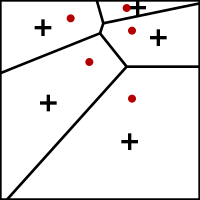
\includegraphics[width=5cm]{lloyd_iterazione_1.png}
\centering
\caption{I iterazione}
\end{figure}

\begin{figure}[H]
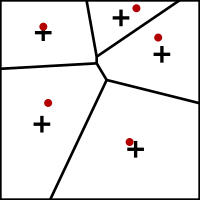
\includegraphics[width=5cm]{lloyd_iterazione_2.png}
\centering
\caption{II iterazione}
\end{figure}

\begin{figure}[H]
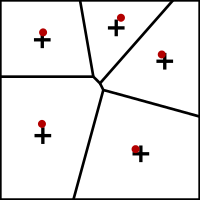
\includegraphics[width=5cm]{lloyd_iterazione_3.png}
\centering
\caption{III iterazione}
\end{figure}

\begin{figure}[H]
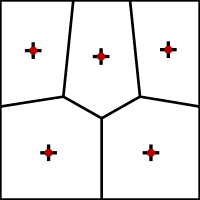
\includegraphics[width=5cm]{lloyd_iterazione_4.png}
\centering
\caption{IV iterazione}
\end{figure}

\subsection{Convergenza dell'algoritmo}

Intuitivamente, si può dire che l'algoritmo converga in quanto i punti che si trovano a minor distanza tra loro tendono a compiere un movimento più alto, mentre i punti che si trovano a distanze elevate tendono a muoversi meno.


\section{Implementazione}

\subsection{Introduzione}

L'implementazione dell'algoritmo di Lloyd richiede una funzione che effettui la tassellazione di Voronoi, la quale a sua volta utilizza una serie di funzioni geometriche che operino nello spazio bidimensionale.

Nell'implementazione che verrà illustrata successivamente, si è scelto di implementare in primo luogo l'algoritmo utilizzando il linguaggio \textit{Python} per avere a disposizione una maggior quantità di strumenti di debugging e testing; successivamente è stato effettuato il porting del codice in \textit{OpenModelica} 

\subsection{Funzioni e classi geometriche}

\subsubsection{Point}

Per poter operare nello spazio bidimensionale, è necessario definire una classe \textit{Point} rappresentante una tupla \textit{x, y}

\begin{lstlisting}[language=Modelica]
record Point
  Real x;
  Real y;
end Point;
\end{lstlisting}

\subsubsection{Verifica della sovrapposizione di due punti}

Può verificarsi che, in seguito a ..., ci si trovi nella situazione in cui due punti sovrapposti non superino il test di equalità. Ad esempio:
\[
P_1 = (4.0, 2.0),
P_2 = (4.00001, 1.999999)
\]

è chiaro come i due punti siano in realtà sovrapposti, ed è quindi necessario definire una funzione che si occupi di verificarlo

\begin{lstlisting}[language=Modelica]
function points_are_close
  input Point p1;
  input Point p2;
  output Boolean out;
protected
  parameter Real tolerance = 0.001;
algorithm
  if abs(p1.x - p2.x) < tolerance then
    if abs(p1.y - p2.y) < tolerance then
      out := true;
    else
      out := false;
    end if;
  else
    out := false;
  end if;
end points_are_close;
\end{lstlisting}

Il valore \textit{tolerance} può essere variato dipendentemente dalla precisione richiesta e dalla scala di applicazione. Nel caso in cui si operi in una scala metrica, ovvero nel caso in cui \textit{1.0} corrisponda ad \textit{1 metro}, una tolleranza di $0.001$ corrisponde ad \textit{1 millimetro}, ed è quindi considerato un valore accettabile dal momento che i droni hanno delle dimensioni nell'ordine di grandezza delle decine di centrimetri.

\subsubsection{Edge}

Per rappresentare un segmento, viene implementata la classe \textit{Edge}. Ogni Edge è definito come una coppia di punti.

\begin{lstlisting}[language=Modelica]
record Edge
  parameter Point starting;
  parameter Point ending;
end Edge;
\end{lstlisting}

\section*{Bibliografia}

\begin{itemize}
	\item https://en.wikipedia.org/wiki/Lloyd\%27s\_algorithm
	\item github.com/zapateocallisto
\end{itemize}

\end{document}